\documentclass[9pt]{beamer}
\usepackage[sfdefault]{roboto}
\usepackage{styles/fluxmacros}
\usefolder{styles}
\usetheme[style=asphalt]{flux}
%\usepackage{xcolor}
\usepackage{color}
%\usepackage{colortbl}
\usepackage{amsmath}
\usepackage{amssymb}
\usepackage{graphicx}
\usepackage{latexsym}
\usepackage[T1]{fontenc}
\usepackage[utf8]{inputenc}
\usepackage{wrapfig}
\usepackage{siunitx}
\usepackage{times}
\usepackage{tikz}
\usepackage{verbatim}
\usepackage{multimedia}
\usepackage{hyperref}
\usepackage{thumbpdf}
\usepackage{pgf,pgfarrows,pgfnodes,pgfautomata,pgfheaps,pgfshade}
\usepackage{url}
\usepackage{empheq}
\usepackage{fancybox}
\usepackage{esint}
\usepackage{lipsum}
\usepackage{listings}
\usepackage{mathptmx}
\usepackage{helvet}
\usepackage{tikz}%
\usepackage{circuitikz}
\usepackage{csvsimple}
\usepackage{pgfplots}
\usepackage{multimedia}
\usepackage{proba}
\usepackage[absolute,overlay]{textpos}
\usepackage{bibunits}
\usepackage{tcolorbox}
\usepackage{qrcode}
\usepackage[texcoord,
            grid,
            gridunit=mm,
            gridcolor=red!60,
            subgridcolor=black!60]{eso-pic}
\usepackage{enumerate}
\setbeamercovered{transparent}
%% Informations
\usepackage[makeroom]{cancel}
\usepackage{epstopdf}
\usepackage{booktabs}
\epstopdfsetup{outdir=./}
\mode<presentation>
{  
    %\usetheme{PaloAlto}
    %\usecolortheme[named=kugreen]{structure}
    \useinnertheme{progressbar}
    %\usefonttheme{default}
    %\usefonttheme{serif}
    %\setbeamercovered{transparent}
    %\setbeamertemplate{blocks}[rounded][shadow=true]
    %\setbeamertemplate{navigation symbols}[only frame symbol]
}
%
%
%~~~~~~~~~~~~~~~~~~~~~~~~~~~~~~~~~~~~~~~~~~~~~~~~~~~~~~~~~~~~~~~~~~~~~~~~~~~~~~
%~~~~~~~~~~~~~~~~~~~~~~~~~~~~~~~~~~~~~~~~~~~~~~~~~~~~~~~~~~~~~~~~~~~~~~~~~~~~~~
% Informations
\defaultbibliography{main}
%
%
%
\title{Modeling optimal control policies}
\subtitle{in stochastic epidemic models}
\author{Saúl Díaz Infante Velasco}
\institute{CONACYT-UNIVERSIDAD de SONORA}
\date{\today}
\titlegraphic{assets/Society_for_Industrial_and_Applied_Mathematics_(logo).png}
%~~~~~~~~~~~~~~~~~~~~~~~~~~~~~~~~~~~~~~~~~~~~~~~~~~~~~~~~~~~~~~~~~~~~~~~~~~~~~~
%\defaultbibliography{first_day_main}
%\defaultbibliographystyle{abbrv}
%%%%%%%%%%%%%%%%%%%%%%%%%%%%%%%%%%%%%%%%%%%%%%%%%%%%%%%%%%%%%%%%%%%%%%%%%%%%%%%%
\def\Q#1#2{\frac{\partial #1}{\partial #2}}
\usetikzlibrary{arrows,shapes}
\pgfplotsset{compat=1.14}
%%%%%%%%%%%%%%%%%%%%%%%%%%%%%%%%%%%%%%%%%%%%%%%%%%%%%%%%%%%%%%%%%%%%%%%%%%%%%%%%
%-----------------------------ExtrasDeTercerPresentacion
%--------------------------------Fancyboxes-------------------------------------
\definecolor{myblue}{rgb}{.8, .8, 1}
\definecolor{azure(colorwheel)}{rgb}{0.0, 0.5, 1.0}
\definecolor{shadecolor}{cmyk}{0,0,0.41,0}
\newcommand*\mybluebox[1]{%
    \colorbox{myblue}{\hspace{1em}#1\hspace{1em}}
}
\newcommand*\myyellowbox[1]{%
    \colorbox{darkyellow}{\hspace{1em}#1\hspace{1em}}
}
%--------------------------------------------------------------------------
\definecolor{shadecolor}{cmyk}{0,0,0.41,0}
\definecolor{light-blue}{cmyk}{0.25,0,0,0}
\newsavebox{\mysaveboxM} % M for math
\newsavebox{\mysaveboxT} % T for text
\newcommand*\Garybox[2][Example]{%
    \sbox{\mysaveboxM}{#2}%
        \sbox{\mysaveboxT}{\fcolorbox{black}{light-blue}{#1}}%
            \sbox{\mysaveboxM}{%
    \parbox[b][\ht\mysaveboxM+.5\ht\mysaveboxT+.5\dp\mysaveboxT][b]{%
        \wd\mysaveboxM}{#2}%
    }%
    \sbox{\mysaveboxM}{%
        \fcolorbox{black}{shadecolor}{%
        \makebox[\linewidth-10em]{\usebox{\mysaveboxM}}%
        }%
    }%
    \usebox{\mysaveboxM}%
    \makebox[0pt][r]{%
        \makebox[\wd\mysaveboxM][c]{%
            \raisebox{\ht\mysaveboxM-0.5\ht\mysaveboxT
            +0.5\dp\mysaveboxT-0.5\fboxrule}{\usebox{\mysaveboxT}}%
        }%
    }%
}
\newcommand\Fontvi{\fontsize{7}{7.2}\selectfont}
%%%%%%%%%%%%%%%%%%%%%%%%%%%%%%%%%%%%%%%%%%%%
\definecolor{kugreen}{RGB}{50,93,61}
\definecolor{kugreenlys}{RGB}{132,158,139}
\definecolor{kugreenlyslys}{RGB}{173,190,177}
\definecolor{kugreenlyslyslys}{RGB}{214,223,216}
\definecolor{greenArea}{RGB}{124,252,124}
\definecolor{hellmagenta}{rgb}{1,0.75,0.9}
\definecolor{hellcyan}{rgb}{0.75,1,0.9}
\definecolor{hellgelb}{rgb}{1,1,0.8}
\definecolor{colKeys}{rgb}{0,0,1}
\definecolor{colIdentifier}{rgb}{0,0,0}
\definecolor{colComments}{rgb}{1,0,0}
\definecolor{colString}{rgb}{0,0.5,0}
\definecolor{darkyellow}{rgb}{1,0.9,0}
\setbeamercovered{transparent}
\lstset{%
    language=[AlLaTeX]TEX,%
    float=hbp,%
    basicstyle=\ttfamily\small, %\usepackage{cir}
    identifierstyle=\color{colIdentifier}, %
    keywordstyle=\color{colKeys}, %
    stringstyle=\color{colString}, %
    commentstyle=\color{colComments}, %
    columns=flexible, %
    tabsize=3, %
    frame=single, %
    extendedchars=true, %
    showspaces=false, %
    showstringspaces=false, %
    numbers=left, %
    numberstyle=\tiny, %
    breaklines=true, %
    backgroundcolor=\color{hellgelb}, %
    breakautoindent=true, %
    captionpos=b,%
    xleftmargin=18pt,%
    xrightmargin=\fboxsep%
}
\pgfplotsset{
    left segments/.code={\pgfmathsetmacro\leftsegments{#1}},
    left segments=3,
    left/.style args={#1:#2}{
        ybar interval,
        domain=#1:#2,
        samples=\leftsegments+1,
        x filter/.code=\pgfmathparse{\pgfmathresult}
       }
}
\DeclareMathOperator{\sign}{sgn}
\newcommand{\innerprod}[2]{\left\langle#1, #2\right\rangle}
\newcommand\bound{10} % bound number of points on each side of N
\newcommand\labelnum[3][]{
    \begin{scope}[font=\footnotesize,x=.3cm,#1]
      \foreach \mypt in {0,#2,...,\bound}{
        \draw(\mypt,0)circle[radius=2pt];
        \draw(-\mypt,0)circle[radius=2pt];
      }
      \draw(-\bound-5,0)--(\bound+5,0) node[pos=0, left]{$t$};
      \node(start)[at={(-\bound-4,0)},label=below:{$t_0=0$}]{$[$};
      \node(end)[at={(\bound+4,0)},label=below:{$T=Nh$}]{$]$};
      \node[%
          at={($(start)!.319!(end)$)},
          label=below:{
               $\underbrace{}_{h}$
            }%
            ]{\vphantom{$[$}};
      \node[at={($(start)!.57!(end)$)},label=below:{$t_{n+1}$}]{\vphantom{$[$}};
      \filldraw(0,0)circle[radius=2pt];
      \node[at={(-\bound-2,0)},above]{$\cdots$};
      \node[at={(\bound+2,0)},above]{$\cdots$};
      \node[at={(0,0)},above=5pt]{#3};
    \end{scope}
}
\usepackage{remreset}
\makeatletter
\@removefromreset{subsection}{section}
\makeatother
\definecolor{greenstrong}{rgb}{0.58,0.77,0.29}
\definecolor{redstrong}{rgb}{0.81,0.22,0.23}
\definecolor{fglisting}{gray}{0.3}
\definecolor{bglisting}{gray}{1}
\definecolor{fgshell}{gray}{1}
\definecolor{bgshell}{gray}{0.1}
\definecolor{bgshelllight}{gray}{0.8}
\definecolor{cadmiumorange}{rgb}{0.93, 0.53, 0.18}
\definecolor{capri}{rgb}{0.0, 0.75, 1.0}
%
\setcounter{subsection}{1}
\newcommand{\hl}[1]{\textbf{\textcolor{greenstrong}{#1}}}
\newcommand{\hb}[1]{\textbf{\textcolor{azure(colorwheel)}{#1}}}
\newcommand{\hlErr}[1]{\textcolor{redstrong}{\texttt{#1}}}
\newcommand{\hlOk}[1]{\textcolor{green}{\texttt{#1}}}
\newcommand{\hlInv}[1]{\colorbox{bgshell}{\textcolor{fgshell}{\texttt{#1}}}}
\newcommand{\unhl}[1]{\textcolor{gray}{#1}}
\newcommand{\clda}[0]{$\textcolor{blue}{\lambda}$}
\newcommand{\carr}[0]{$\textcolor{purple}{\rightarrow}$}
\newcommand{\cbind}[0]{\textbf{\texttt{$>\!\!>\!\!=$}}}
\newcommand{\codedots}[0]{\textcolor{mid-gray}{...}}

%
\tcbuselibrary{skins, breakable}
\newtcolorbox{greenbox}[1]{%
        colback = green!5!white,
        colframe = green!55!black,
        fonttitle = \bfseries,
        title = #1 %
    }
\newtcolorbox{bluebox}[1]{%
        colback = blue!5!white,
        colframe = blue!55!black,
        fonttitle = \bfseries,
        title = #1
    }
%
\newtcolorbox{graybox}[1]{%
        colback = gray!5!white,
        colframe = gray!55!black,
        fonttitle = \bfseries,
        title = #1
    }
%
\newtcolorbox{yellowbox}[1]{%
        colback = yellow!5!white,
        colframe = yellow!55!black,
        fonttitle = \bfseries,
        title = #1
    }

\begin{document}
    \titlepage
    \section{Introduction}
        \begin{frame}{Tomato leaf curl virus disease (TYLCVD)}
    \only<1>{
        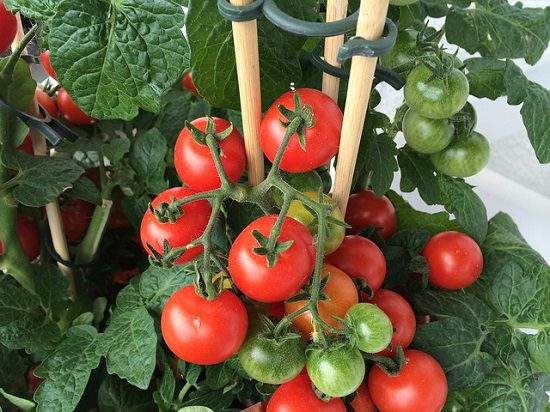
\includegraphics[width=0.7\textwidth,keepaspectratio]{assets/healty_leaf}
    }
    \only<2>{
        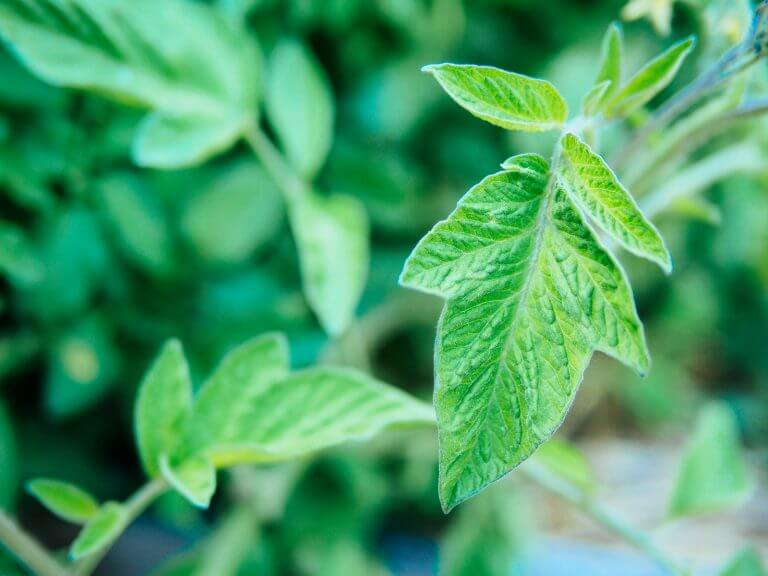
\includegraphics[width=0.7\linewidth]{assets/healty_tomato_leaf}
    }
\end{frame}
%%%%%%%%%%%%%%%%%%%%%%%%%%%%%%%%%%%%%%%%%%%%%%%%%%%%%%%%
\begin{frame}{Tomato leaf curl virus disease (TYLCVD)}
    \begin{textblock*}{65mm}(73mm, 10mm)
        \only<1->{
            \includegraphics[scale=0.08,%
                keepaspectratio]{assets/TYLCV_leaflet_cropped}
        }
    \end{textblock*}
    \begin{textblock*}{60mm}(5mm, 10mm)
        \begin{greenbox}{}
            \begin{itemize}[<+->]
                \item
                    Tomato plants \hl{infected early}
                    are severely stunted and will
                    \hl{not produce fruit}
                \item
                    Leaflets are small and yellowed 
                    with edges that curl upwards
                \item
                    Flowers either do not develop or 
                    fall off
                \item
                    When \hl{older plants} are 
                    infected, fruit that is already
                    forming ripens normally, but 
                    \hl{no new fruit} 
                    is formed after the infection
                \item
                    TYLCV can be confused with several 
                    other conditions such as tomato big 
                    bud, herbicide damage and phosphate 
                    or magnesium deficiency
            \end{itemize}
        \end{greenbox}
    \end{textblock*}
 \end{frame}
%%%%%%%%%%%%%%%%%%%%%%%%%%%%%%%%%%%%%%%%%%%%%%%%%%%%%%%%
\begin{frame}{Tomato leaf curl virus disease (TYLCVD)}
    \begin{textblock*}{60mm}(67mm, 30mm)
        \only<1-4>{
        \includegraphics[width=\linewidth]{assets/Silverleaf_whitfly_large_rotated}
        }
        \only<5-6>{
        \includegraphics[width=\linewidth]{assets/ibicum_rosanensis}    
    }
    \end{textblock*}
    \begin{textblock*}{55mm}(10mm, 10mm)
        \begin{greenbox}{Spread}
            \begin{itemize}[<+->]
                \item
                    \hl{TYLCV} is spread by the insect 
                    silverleaf whitefly (Bemisia tabaci 
                    B biotype)
                \item
                    Silverleaf whiteflies pick up the 
                    virus by feeding on infected host 
                    plants. The whiteflies then 
                    spread the virus to healthy plants 
                    \hl{ which show the symptoms 
                    10 to 21 days later}
                \item
                    Silverleaf whiteflies are 
                    \hl{common} in many countries and 
                    \hl{feed} on \hl{many} types of 
                    \hl{plants}
                \item
                    More than 22 species,
                    including both annuals and perennials, are also
                    known hosts of TLCV.
            \end{itemize}
        \end{greenbox}
    \end{textblock*}
\end{frame}
%%%%%%%%%%%%%%%%%%%%%%%%%%%%%%%%%%%%%%%%%%%%%%%%%%%%%%%%
%%%%%%%%%%%%%%%%%%%%%%%%%%%%%%%%%%%%%%%%%%%%%%%%%%%%%%%%
\begin{frame}{}
    \begin{textblock*}{55mm}(5mm, 2mm)
        \begin{bluebox}{Control}
            Cultural Control
            \begin{itemize}[<+->]
                \item
                    Physical barriers
                \item
                    Planting dates
                \item
                    \textbf{Removal of infested plants}
                \item
                    Host plant resistance
            \end{itemize}
            Biological Control
            \tcblower
            \begin{itemize}[<+->]
                \item
                    Parasitoids
                \item
                    Predators
                \item
                    Fungi
            \end{itemize}
        \end{bluebox}
    \end{textblock*}
%
    \begin{textblock*}{60mm}(65mm, 2mm)
        \begin{yellowbox}{Insecticides}
            \begin{itemize}
                \item 
                    pymetrozine
                 \item 
                    zeta-cypermethrin / bifenthrin
            \end{itemize}
        \end{yellowbox}
        \begin{graybox}{}
            \begin{bibunit}[apalike]
                \nocite{Shun-xiang2001}
                \nocite{Smith2014}
                \putbib
            \end{bibunit}
        \end{graybox}
    \end{textblock*}
\end{frame}

    \begin{frame}
        \frametitle{Table of contents}
        \tableofcontents
    \end{frame}
    \section{Deterministic optimal policies}
        \begin{frame}{}
    \begin{textblock*}{60mm}(0mm, 0mm)
        \begin{bibunit}
            \nocite{Holt1999}
            \putbib
        \end{bibunit}
    \end{textblock*}
%
    \begin{textblock*}{70mm}(55mm,15mm)
        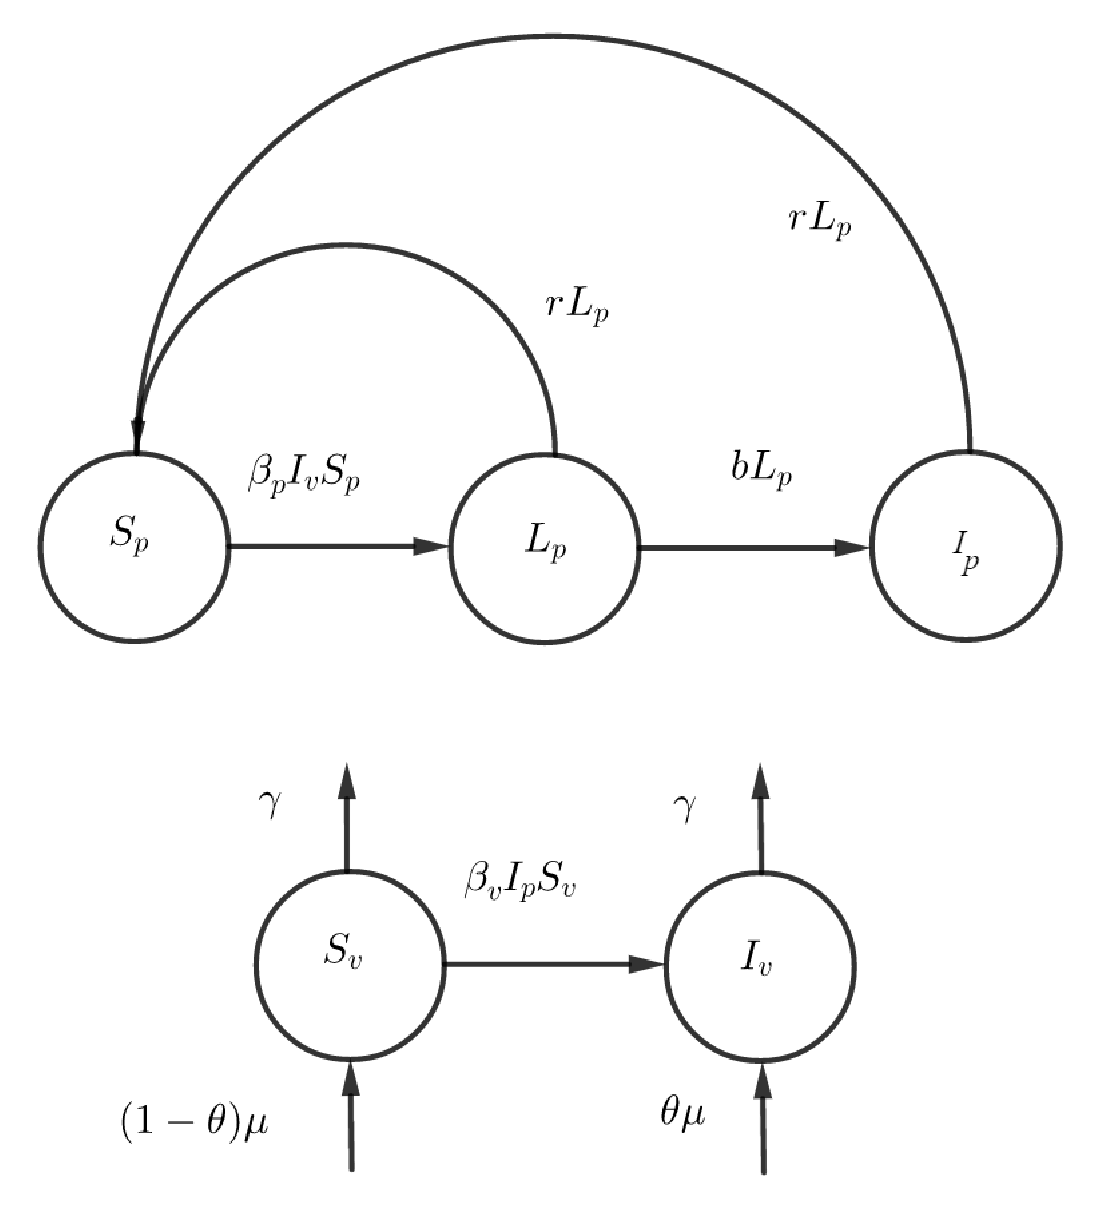
\includegraphics[width=\linewidth]{assets/deterministic_model_diagram.eps}
    \end{textblock*}
    \begin{textblock*}{50mm}(2mm,25mm)
        \begin{graybox}{Hypothesis:}
            \begin{itemize}[<+->]
                \item Remove from latent and infected plants,
                \item plants become latent plants by infected vectors,
                \item latent plants become infectious plants,
                \item vectors become infected vectors by infected plants,
                \item vectors die per day,
                \item immigration from alternative hosts.
            \end{itemize}
        \end{graybox}
    \end{textblock*}
\end{frame}
%%%%%%%%%%%%%%%%%%%%%%%%%%%%%%%%%%%%%%%%%%%%%%%%%%%%%%%%%%%%%%%%%%%%%%%%%%%%%%%%
\begin{frame}{}
    \begin{textblock*}{55mm}(2mm, 5mm)
        \begin{bluebox}{}
            \begin{align*}
                \frac{dS_p}{dt} &=
                    -\beta_p S_p I_v + 
                    \textcolor<2->{azure(colorwheel)}{\textbf<2>{r}}
                    (L_p + I_p)
                    \\
                \frac{dL_p}{dt} &=
                    \beta_p S_p I_v -b L_p -
                    \textcolor<2->{azure(colorwheel)}{\textbf<2>{r}}
                    L_p
                    \\
                \frac{dI_p}{dt} &=
                     b L_p -
                    \textcolor<2->{azure(colorwheel)}{\textbf<2>{r}}
                    I_p
                    \\
                \frac{dS_v}{dt} &=
                    -\beta_v S_v I_p - 
                    \textcolor<2->{cadmiumorange}{\gamma}
                    S_v + (1-\theta)\mu
                    \\
                \frac{dI_v}{dt} &=
                    \beta_v S_v I_p - 
                    \textcolor<2->{cadmiumorange}{\gamma} I_v 
                    + \theta\mu
            \end{align*}
        \end{bluebox}
    \end{textblock*}
%%%%%%%%%%%%%%%%%%%%%%%%%%%%%%%%%%%%%%%%%%%%%%%%%%%%%%%%%%%%%%%%%%
    \begin{textblock*}{45mm}(3mm, 55mm)
        \begin{empheq}[box=\shadowbox]{align*}
            R_0 &=
                \sqrt{\frac{\beta_v\mu 
                b\beta_p}{r^2(r+b)\gamma}}
            \\
            DFE &= 
                (N_p, 0, 0, 0,  \mu / \gamma)^{\top}
            \\
            EE &=
                (S_p ^ *, L_p ^ *, I_p ^ *, S_v ^ *, I_v ^ * ) ^ {\top}
        \end{empheq}
    \end{textblock*}
    \begin{textblock*}{60mm}(65 mm, 5mm)
        \begin{tabular}{@{}lll@{}} 
            \toprule
            Par. & Value & Descrip. 
            \\ 
            \midrule
                $\beta_p$ 
                & 0.1 
                & latent rate  
            \\ 
                $r$ 
                & 0.01 
                & remove rate 
            \\
                $1/b$ 
                & 0.075 
                & time of latency
            \\
                $\gamma$ 
                & 0.06 
                & vector die or depart rate 
            \\
                $\mu$ 
                & 0.3 
                & immigration rate 
            \\
                $\theta$ 
                & 0.2 
                & infected vectors 
                    arrival 
                \\
                $\beta_v$ 
                & 0.003 
                & vector infected 
                rate
            \\
            \bottomrule
        \end{tabular}
    \end{textblock*}
    \begin{textblock*}{70mm}(57mm, 50mm)
        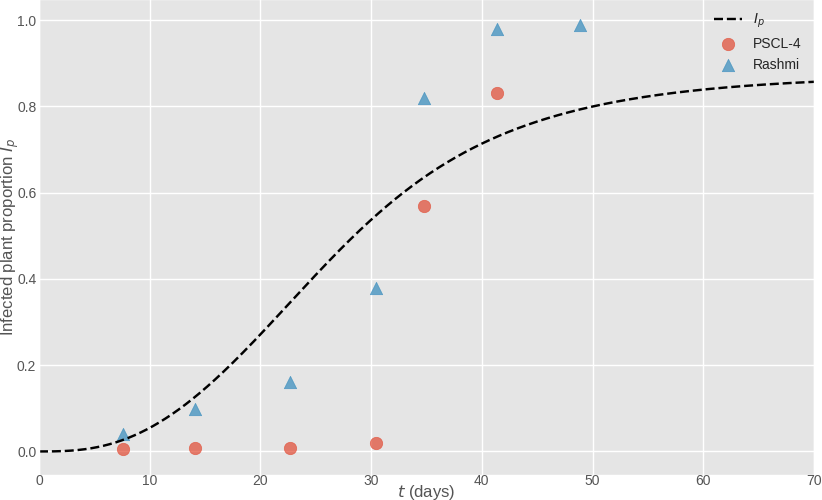
\includegraphics[width=\linewidth]{assets/data_dynamics_jegger}
    \end{textblock*}
\end{frame}
        \begin{frame}{Deterministic controlled dynamics}
    \begin{textblock*}{63mm}(2mm, 12mm)
        \begin{bluebox}{}
            \only<1-2>{
                \begin{align*}
                    \frac{dS_p}{dt} &=
                        -\beta_p S_p I_v + 
                        \textcolor{azure(colorwheel)}{\textbf{r}}
                        (L_p + I_p)
                        \\
                    \frac{dL_p}{dt} &=
                        \beta_p S_p I_v -b L_p -
                        \textcolor{azure(colorwheel)}{\textbf{r}}
                        L_p
                        \\
                    \frac{dI_p}{dt} &=
                         b L_p -
                        \textcolor{azure(colorwheel)}{\textbf{r}}
                        I_p
                        \\
                    \frac{dS_v}{dt} &=
                        -\beta_v S_v I_p - 
                        \textcolor{cadmiumorange}{\gamma}
                        S_v + (1-\theta)\mu
                        \\
                    \frac{dI_v}{dt} &=
                        \beta_v S_v I_p - 
                        \textcolor{cadmiumorange}{\gamma} I_v 
                        + \theta\mu
                \end{align*}
            }
            \only<3->{
                \begin{align*}
                    \frac{dS_p}{dt} &=
                        -\beta_p S_p I_v + 
                        \textcolor{azure(colorwheel)}{
                            (u_1 + r) 
                        } L_p 
                        + 
                        \textcolor{azure(colorwheel)}{
                            (u_2 + r)
                        } I_p
                        \\
                    \frac{dL_p}{dt} &=
                        \beta_p S_p I_v -b L_p -
                        \textcolor{azure(colorwheel)}{(u_1 + r)} L_p
                        \\
                    \frac{dI_p}{dt} &=
                         b L_p -
                        \textcolor{azure(colorwheel)}{(u_2 + r)} I_p
                        \\
                    \frac{dS_v}{dt} &=
                        -\beta_v S_v I_p - 
                        \textcolor{cadmiumorange}{(\gamma + u_3)}
                        S_v + (1-\theta)\mu
                        \\
                    \frac{dI_v}{dt} &=
                        \beta_v S_v I_p - 
                        \textcolor{cadmiumorange}{(\gamma + u_3)} I_v 
                        + \theta\mu
                \end{align*}
            }
        \end{bluebox}
    \end{textblock*}
    \begin{textblock*}{55mm}(2mm, 65mm)
        \begin{yellowbox}{}
            \begin{align*}
                u_1(t)&:
                    \text{ Latent replanting}
                \\
                u_2(t)&:
                    \text{ Infected replanting}
                \\
                u_3(t)&:
                    \text{ Fumigation}
            \end{align*}
        \end{yellowbox}
    \end{textblock*}
    %%%%%%%%%%%%%%%%%%%%%%%%%%%%%%%%%%%%%%%%%%%%%%%%%%%%%%%%%%%%%%%%%%%%%%%%%%%%
    \begin{textblock*}{58mm}(60mm, 65mm)
        \begin{align*}
            \int_{0}^T
                \left[
                A_1 I_p(t) + A_2 L_p(t) + A_3 I_v(t)
                + \sum_{i=1}^3
                    c_i \frac{u_i ^ 2}{2}
                \right] dt
        \end{align*}
    \end{textblock*}
\end{frame}
    \section{Existence of deterministic optimal Policies}
        \begin{frame}
    %\frametitle{Existence Theory}
    \begin{textblock*}{60mm}(1mm,5mm)
        \begin{greenbox}{Consider the controlled dynamics}
            $$\left\{ \begin{array}{l}
                \dot{x}(s)=f(s,u(s),x(s))\,\,s\in [t_0,T], \\
            x(t_0)=x_0,\\
            \end{array}
        \right.$$
        \tcblower
        with terminal state constraint
        $$x(T;t_0,x_0,u(\cdot))\in M, M\subseteq \mathbb{R}^n.$$
        \end{greenbox}
    \end{textblock*}
    \begin{textblock*}{65mm}(2mm, 50mm)
        \begin{yellowbox}{Cost functional}
           \hspace{-3mm}
           ${
               \tilde{\mathcal{U}}_{x_0}[t_0,T]
               :=
               \left\{%
                   u:[t_0, T]\to \mathbb{R}^n
                   | \text{ measurable}
               \right\}
           }
           $%
           \begin{align*}
                J(t_0,x_0;u(\cdot))
                   =&
                    \int_{t_0}^{T}
                       g(s, u(s), x(s)) ds
                   \\
                       &+ h(T, x(T))
           \end{align*}
        \end{yellowbox}
    \end{textblock*}
    \begin{textblock*}{65mm}(62mm,5mm)
        \begin{graybox}{Problem $(OC)$}
            $
            {
                (t_0,x_0)
                \in \mathbb{R}_{+}\times \mathbb{R}^n
            }
            $ , 
            find a control policie
            $
                {
                \bar{u}(\cdot)\in 
                \tilde{\mathcal{U}}_{x_0}[t_0,T]
                }
            $ 
            s.t.
            \begin{equation*}
                J(t_0, x_0; \bar{u}(\cdot))=
                    \inf_{u(\cdot)  \in 
                \tilde{\mathcal{U}}_{x_0}[t_0,T]} 
                J(t_0,x_0;u(\cdot)).
            \end{equation*}
        \end{graybox}
\end{textblock*}
\end{frame}
%%%%%%%%%%%%%%%%%%%%%%%%%%%%%%%%%%%%%%%%%%%%%%%%%%%%%%%%%%%%%%%%%%%%%%%%%%%%%%%%

\begin{frame}[plain]
    \begin{textblock*}{60mm}(5mm,5mm)
        \begin{graybox}{Hypothesis:}
            \begin{enumerate}[(\textbf{{C}}-1)]
                \item<1->
                    $
                        f:\mathbb{R}_{+}\times U
                        \times \mathbb{R}^n\rightarrow 
                        \mathbb{R}^n
                    $ is measurable, satisfies the lipchitz
                    condition in $x$,
                    $
                        |f(t,u,0)|\leq L,\,
                    \forall\,(t,u)\in
                    \mathbb{R}_{+}\times U .
                    $
                \item<2->
                   $
                        g:\mathbb{R}_{+}\times U\times 
                        \mathbb{R}^n\rightarrow \mathbb{R},
                   $ 
                   $
                        h:\mathbb{R}^n\rightarrow \mathbb{R}
                   $ are measurable, and
                   \begin{align*}
                        &|g(s,u,x_1)-g(s,u,x_2)|+\\
                        &|h(x_1)-h(x_2)|\\
                        &\leq \omega(|x_1|\vee |x_2|,|x_1-x_2|)
                    \end{align*}
                    $
                        \forall\, (s,u)\in \mathbb{R}_{+}
                        \times U,x_1,x_2\in \mathbb{R}^n
                    $.
                \item<3->
                    For a.a. $t\in[0,T]$, 
                    Cesari property holds $\forall$ $x\in 
                    \mathbb{R}^n$.
                \end{enumerate}	
        \end{graybox}
    \end{textblock*}
        \only<2->{
            \begin{textblock*}{55mm}(70mm,5mm)
                \begin{yellowbox}{Modulus of continuity}
                    $
                        \omega:\mathbb{R}_{+}
                        \times\mathbb{R}_{+}\rightarrow 
                        \mathbb{R}_{+}
                    $, 
                    {increasing}, 
                   $\omega(r,0)=0$ $\forall r\geq 0$.
                \end{yellowbox}
            \end{textblock*}
        }
        \only<3>{
            \begin{textblock*}{55mm}(70mm,30mm)
                \begin{yellowbox}{Cesari property}
                    \begin{align*}
                        &
                        \mathbf{E}(t,x)
                             =\{(z^0,z)\in \mathbb{R}\times 
                            \mathbb{R}^n|
                        \\
                        &z^0\geq g(t,u,x),
                        \\
                        &z=f(t,u,x),\, u\in U\}.
                    \end{align*}
                    \tcblower
                    \begin{equation*}
                        \bigcap_{\delta}\bar{co}
                        \mathbf{E}(t,B_{\delta}(x))=\mathbf{E}(t,x)
                    \end{equation*}	
            \end{yellowbox}
        \end{textblock*}
    }
\end{frame}
%%%%%%%%%%%%%%%%%%%%%%%%%%%%%%%%%%%%%%%%%%%%%%%%%%%%%%%%%%%%%%%%%%%%%%%%%%%%%%%%

\begin{frame}[plain]
	\begin{textblock*}{60mm}(5mm,5mm)
		\begin{graybox}{Hypothesis:}
			\begin{enumerate}[(\textbf{{C}}-1)]
				\item
					$
					f:\mathbb{R}_{+}\times U
					\times \mathbb{R}^n\rightarrow 
					\mathbb{R}^n
					$ is measurable, satisfies a lipchitz
					condition in $x$,
					$
					|f(t,u,0)|\leq L,\,
					\forall\,(t,u)\in
					\mathbb{R}_{+}\times U .
					$
				\item
					$
					g:\mathbb{R}_{+}\times U\times 
					\mathbb{R}^n\rightarrow \mathbb{R},
					$ 
					$
					h:\mathbb{R}^n\rightarrow \mathbb{R}
					$ are measurable, and
					\begin{align*}
					&|g(s,u,x_1)-g(s,u,x_2)|+\\
					&|h(x_1)-h(x_2)|\\
					&\leq \omega(|x_1|\vee |x_2|,|x_1-x_2|)
					\end{align*}
					$
					\forall\, (s,u)\in \mathbb{R}_{+}
					\times U,x_1,x_2\in \mathbb{R}^n
					$.
				\item
					For a.a. $t\in[0,T]$, Cesari property holds $\forall$ $x\in 
					\mathbb{R}^n$.
			\end{enumerate}	
		\end{graybox}
	\end{textblock*}


	
	\begin{textblock*}{55mm}(70mm,15mm)
		\begin{graybox}{Existence Theorem}
			Let (C1)-(C3) hold. Then problem $(OC)$ admits at least one optimal 
			pair.
		\end{graybox}
	\end{textblock*}
\end{frame}
    \section{Characterization of optimal policies}
        \begin{frame}[plain]
    \frametitle{Optimal Control Characterization}
    \begin{textblock*}{65mm}(1mm,15mm)
        \begin{yellowbox}{$(OC)^T$}
            \begin{multline*}
                J(t_0,x_0;u(\cdot))
                    = \int_{t_0}^{T} g(s,u(s),x(s)) ds
                    \\
                         + h(x(T))
            \end{multline*}
            $$
                \left\{ 
                    \begin{array}{l}
                        \dot{x}(s)=f(s,u(s),x(s))\,\,s\in [t_0,T]
                        \\
                        x(t_0)=x_0
                        \\
                    \end{array}
                \right.
            $$
    %
        \end{yellowbox}
    \end{textblock*}
%
    \begin{textblock*}{65mm}(1mm,60mm)
        \begin{greenbox}{Hamiltonian:}
            \begin{equation*}
                H=g(t,x(t),u(t))
                    +\langle \lambda(t),f(t,x(t),u(t))\rangle,
            \end{equation*}
        \tcblower
            \begin{equation*}
                \frac{\partial H}{\partial 
                u_i}(t,\bar{x}(\cdot),\bar{u}(\cdot))=0.
            \end{equation*}
        \end{greenbox}
    \end{textblock*}
    \begin{textblock*}{60mm}(67mm,15mm)
        \begin{graybox}{Additional hypothesis:}
            \begin{enumerate}[(\textbf{{C}}-4)]
                \item
                \hspace*{-2mm}
                \\
                $
                    x \mapsto 
                    \left(
                        f(t,u,x),g(t,u,x),h(x)
                    \right)
                $
                \\
                is differentiable,
                \\
                \begin{multline*}
                    \hspace*{-15mm}
                    (u,x) 
                    \mapsto 
                    (f(t,u,x),f_x(t,u,x),
                    \\
                    g(t,u,x),g_x(t,u,x),
                    \\
                    h_x(x))
                \end{multline*}
                is continuous.
            \end{enumerate}
        \end{graybox}
    \end{textblock*}
\end{frame}
%%%%%%%%%%%%%%%%%%%%%%%%%%%%%%%%%%%%%%%%%%%%%%%%%%%%%%%%%%%%%%%%%%%%%%%%%%%%%%%%%
\begin{frame}[plain]
    \begin{textblock*}{120mm}(5mm,5mm)
        \begin{graybox}{Pontryagin’s Maximum Principle}
            If $\bar{u}(t)$ and $\bar{x}(t)$ are optimal for the problem 
            $(OC)$, then there exists a piecewise differentiable adjoint 
            variable $\lambda(t)$ s.t.
            \begin{equation*}
                H(t,\bar{x}(t), \bar{u(t)}, \lambda(t))
                =
                \max_{u \in U} H(t, x(t), u(t), \lambda(t)),
                \qquad \forall t \in [0, T]
            \end{equation*}
%
            \begin{align*}
                    \lambda'(t) &= -\frac{\partial 
                    H(t,\bar{x}(t),\bar{u}(t),\lambda(t))}{\partial x},\\
                \lambda(T) &= 0.
            \end{align*}
        \end{graybox}
    \end{textblock*}
    \begin{textblock*}{75mm}(5mm,65mm)
        \begin{yellowbox}{Hamiltonian}
            \begin{equation*}
                H=g(t,x(t),u(t))+\langle \lambda(t),f(t,x(t),u(t))\rangle,
            \end{equation*}
        \end{yellowbox}
    \end{textblock*}
\end{frame}
%
%%%%%%%%%%%%%%%%%%%%%%%%%%%%%%%%%%%%%%%%%%%%%%%%%%%%%%%%%%%%%%%%%%%%%%%%%%%%%%%%%
\begin{frame}[plain]
\frametitle{Example}
    \only<1,2>
    {
        \begin{textblock*}{70mm}(1mm,10mm)
            \begin{greenbox}{}
                \begin{align*}
                    \frac{dS_p}{dt} &=
                    -\beta_p S_p I_v +(\textcolor{capri}{r 
                    +u_1})L_p + 
                    (\textcolor{capri}{r + u_2}) I_p,
                    \\
                    \frac{dL_p}{dt} &=
                    \beta_p S_p I_v -b L_p 
                    -(\textcolor{capri}{r + u_1})L_p,
                    \\
                    \frac{dI_p}{dt} &= 
                    b L_p - (\textcolor{capri}{r + u_2}) I_p,
                    \\
                    \frac{dS_v}{dt} &=
                    -\beta_v S_v I_p 
                    - (\textcolor{cadmiumorange}{\gamma+u_3}) 
                    S_v 
                        +(1-\theta)\mu,
                    \\
                    \frac{dI_v}{dt} &=
                    \beta_v S_v I_p 
                    -(\textcolor{cadmiumorange}{\gamma+u_3}) 
                    I_v 
                    +\theta\mu,
                \end{align*}
            \end{greenbox}
        \end{textblock*}
    }
    \only<2>{
        \begin{textblock*}{55mm}(72mm,10mm)
            \begin{greenbox}{}
                \begin{align*}
                    H
                            &=A_1I_v+A_2L_p+A_3I_v
                        \\
                        &+\sum_{i=1}^{3}c_iu_i^2
                        \\
                            &
                        +\textcolor{colComments}{\lambda_1}(-\beta_p
                         S_p I_v 
                        +(r +u_1)L_p\\
                        &+ (r + u_2) I_p)
                        \\
                        &+\textcolor{colComments}{\lambda_2}(\beta_p
                         S_p I_v -b 
                        L_p
                        \\
                        &-(r + u_1)L_p)\\
                        &+\textcolor{colComments}{\lambda_3}(b
                         L_p - (r + u_2) 
                        I_p
                        )\\
                        &+\textcolor{colComments}{\lambda_4}(-\beta_v
                         S_v I_p - 
                        (\gamma+u_3) S_v\\ &+(1-\theta)\mu)
                        \\
                        &+\textcolor{colComments}{\lambda_5}(\beta_v
                         S_v I_p 
                        -(\gamma+u_3) I_v
                        \\
                        & +\theta\mu).
                \end{align*}
            \end{greenbox}
        \end{textblock*}
    }
\end{frame}%
%%%%%%%%%%%%%%%%%%%%%%%%%%%%%%%%%%%%%%%%%%%%%%%%%%%%%%%%%%%%%%%%%%%%%%%%%%%%%%%%%
\begin{frame}[plain]
    \begin{textblock*}{80mm}(5mm,2mm)
        \begin{greenbox}{}
            \begin{align*}
                \frac{d\lambda_1}{dt} 
                    &=
                    \beta_p (\lambda_1-\lambda_2),
                \\
                \frac{d\lambda_2}{dt} 
                    &=-A_2+(r+u_1)(\lambda_2-\lambda_1)
                    +b (\lambda_2-\lambda_3),
                \\
                \frac{d\lambda_3}{dt} 
                    &=
                    - A_1 + (r+u_2)(\lambda_3-\lambda_1)
                     + \beta_v S_v (\lambda_4-\lambda_5),
                \\
                \frac{d\lambda_4}{dt} 
                    &=
                    \beta_v I_p (\lambda_4-\lambda_5)
                    + (\gamma+u_3) \lambda_4,
                \\
                \frac{d\lambda_5}{dt} 
                    &=
                    -A_3+\beta_p  S_p(\lambda_1-\lambda_2)
                    + (\gamma+u_3)\lambda_5,
            \end{align*}
        \end{greenbox}
    \end{textblock*}
%
    \begin{textblock*}{32mm}(10mm,70mm)
        \begin{yellowbox}{}
            $\frac{\partial H}{\partial u}(\bar{u})=0 
            \Rightarrow$
            \tcblower
            $
                u_i \in 
                [0, u_i^{max}]
            $
        \end{yellowbox}
    \end{textblock*}
%
    \begin{textblock*}{70mm}(50mm,52mm)
        \begin{yellowbox}{optimal control policies}
            \begin{align*}
                \bar{u}_1
                    &=
                    \min
                        \left(
                            \max
                                \left(
                                    0,
                                    \frac{L_p(\lambda_2-\lambda_1)}{2c_1}
                                \right),
                            u_1^{max}
                        \right)
                \\
                \bar{u}_2
                    &=
                    \min
                        \left(
                            \max
                                \left(
                                    0,\frac{I_p(\lambda_3-\lambda_1)}{2c_2}
                                \right),
                                u_2^{max}
                        \right)
                        \\
                \bar{u}_3
                    &=
                    \min
                        \left(
                            \max
                                \left(
                                    0,\frac{S_v\lambda_4+I_v\lambda_5}{2c_3}
                                \right), 
                                u^{max}_3
                        \right)
            \end{align*}
        \end{yellowbox}
    \end{textblock*}
\end{frame}
%%%%%%%%%%%%%%%%%%%%%%%%%%%%%%%%%%%%%%%%%%%%%%%%%%%%%%%%%%%%%%%%%%%%%%%%%%%%%%%%%

    \section{Numeric Results}
        \begin{frame}{The most popular}
    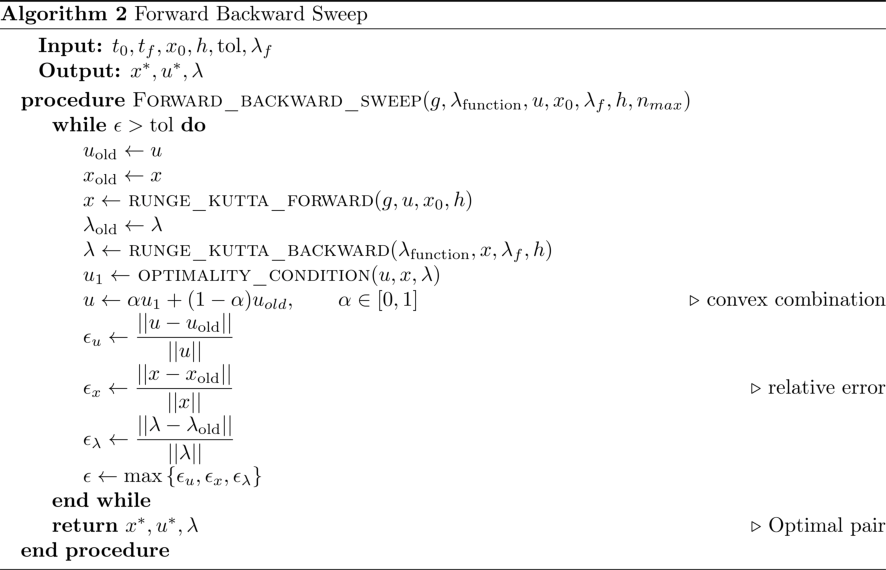
\includegraphics[width=1\linewidth]{assets/fbs_algorithm.pdf}
\end{frame}
%%%%%%%%%%%%%%%%%%%%%%%%%%%%%%%%%%%%%%%%%%%%%%%%%%%%%%%%%%%%%%%%%%%%%%%%%%%%%%%%
\begin{frame}
    \frametitle{Control by fumigation}
    \begin{center}
        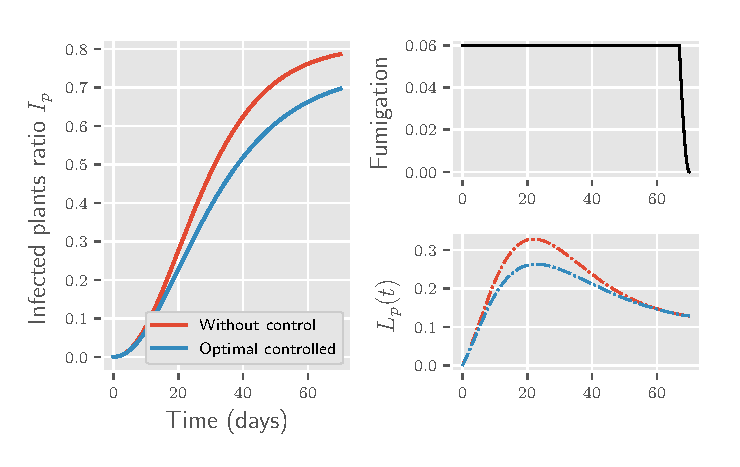
\includegraphics{numerical_results/figure_1_tylc_only_control_fumigation}
    \end{center}
\end{frame}
%
\begin{frame}
    \frametitle{Control by replanting infected plants}
    \begin{center}
        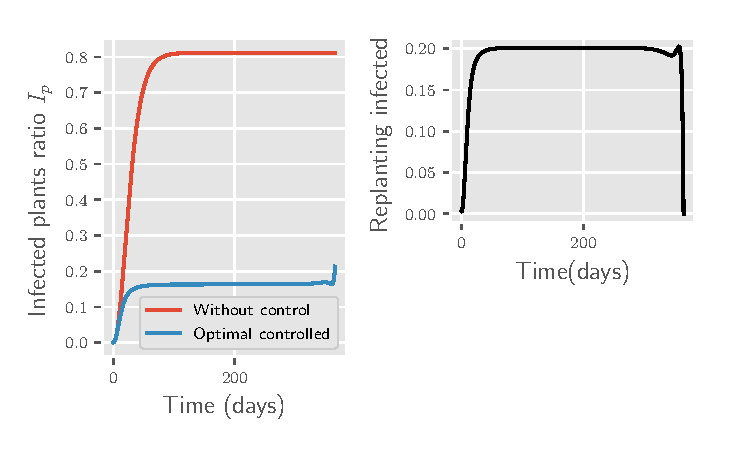
\includegraphics{numerical_results/figure_1_tomato_controlled_by_replanting_infected}
    \end{center}
\end{frame}
%%%%%%%%%%%%%%%%%%%%%%%%%%%%%%%%%%%%%%%%%%%%%%%%%%%%%%%%%%%%%%%%%%%%%%%%%%%%%%%%
\begin{frame}
    \frametitle{Control by replanting and fumigation}
    \begin{center}
        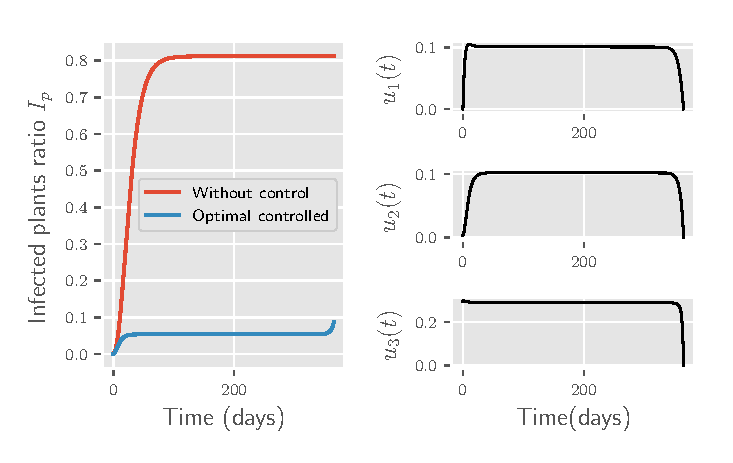
\includegraphics{numerical_results/figure_1_tomato_replanting_and_fumigation}
    \end{center}
    
\end{frame}
%%%%%%%%%%%%%%%%%%%%%%%%%%%%%%%%%%%%%%%%%%%%%%%%%%%%%%%%%%%%%%%%%%%%%%%%%%%%%%%%
\begin{frame}
    \frametitle{Control by replanting}
    \begin{center}
        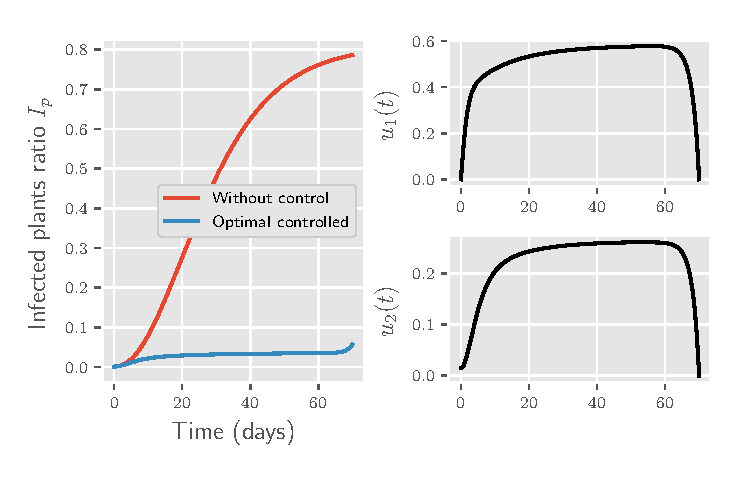
\includegraphics{numerical_results/figure_1_tomato_control_replanting}
    \end{center}
\end{frame}
%%%%%%%%%%%%%%%%%%%%%%%%%%%%%%%%%%%%%%%%%%%%%%%%%%%%%%%%%%%%%%%%%%%%%%%%%%%%%%%%
\begin{frame}{Control cost likening}
    \begin{center}
        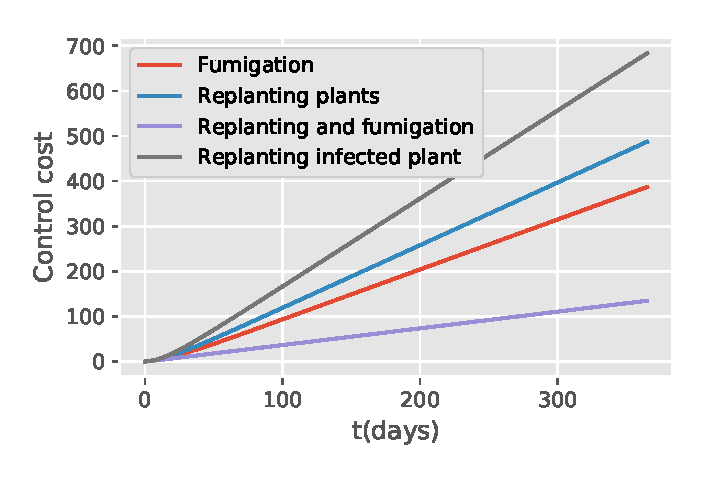
\includegraphics{numerical_results/control_cost}
    \end{center}
\end{frame}

    \section{Stochastic extension}
        \begin{frame}[plain]
    \frametitle{Stochastic optimal control theory}
    \begin{textblock*}{100mm}(15mm,10mm)
        \begin{graybox}{Set up}
            \begin{align*}
                (\Omega, & \mathcal{F}, \{\mathcal{F}_t\}_{t\geq 0}, \mathbb{P})
                \\
                W(t)&: m\text{-dimensional Brownian motion}
                \\
                dx(t)&=
                    f(t,u(t),x(t))dt+\sigma(t,u(t),x(t))dW(t)
                \\
                x(0)&=x_0,
                \\
                f &:
                    [0,T]\times U \times \mathbb{R}^n 
                    \to \mathbb{R}^n, 
                \\
                \sigma &: [0,T]\times U \times \mathbb{R}^n
                \to\mathbb{R}^{n+m},
                \\
                U &: \text{separable metric space}.
            \end{align*}
            \tcblower
            $
                \mathcal{U}[0,T]:=
                    \{
                        u:[0,T]\times\Omega 
                        \to U |
                         u(\cdot)\, 
                         \text{is}\, 
                         \{\mathcal{F}_t\}_{t\geq 0}\text{-adapted}
                    \}
            $
        \end{graybox}
    \end{textblock*}
\end{frame}
%%%%%%%%%%%%%%%%%%%%%%%%%%%%%%%%%%%%%%%%%%%%%%%%%%%%%%%%%%%%%%%%%%%%%%%%%%%%%%%%%
\begin{frame}[plain]
    \begin{textblock*}{90mm}(20mm,15mm)
        \begin{graybox}{Weak formulation of optimal control}
             A 6-tuple 
             $
                \pi=(
                    \Omega,
                    \mathcal{F},
                    \{\mathcal{F}_t\}_{t\geq 0},
                    \mathbb{P},
                    W(\cdot),
                    u(\cdot)
                )
            $, 
            is  a {w-admissible} control, if
        \begin{itemize}[<+->]
            \item 
                $
                    (
                        \Omega,
                        \mathcal{F},
                        \{\mathcal{F}_t\}_{t\geq 0},
                        \mathbb{P}
                    )
                $ is a filtered probability space satisfying the usual
                conditions,
            \item 
                $W(t)$ 
                is an $m$-dimensional standard Brownian motion 
                defined on 
                $
                    (
                        \Omega,
                        \mathcal{F},
                        \{\mathcal{F}_t\}_{t\geq 0},\mathbb{P}
                    )
                $,
            \item 
                $u(\cdot)$ is an 
                $
                    \{
                        \mathcal{F}_t\}_{t \geq 0}
                        \text{-adapted}
                $ 
                process on $(\Omega,\mathcal{F},\mathbb{P})$ taking values 
                in $U$,
            \item 
                $x(\cdot)$ is unique solution,
            \item 
                some prescribed state constraints are satisfied,
            \item 
                $
                    g(\cdot, u(\cdot), x(\cdot))
                    \in 
                    L^1_{
                        \mathcal{F}
                    }
                    (
                        0, T; \mathbb{R}
                )
                $ and 
                $
                    h(x(T))
                    \in 
                    L^1_{\mathcal{F}_T}
                    (\Omega;\mathbb{R})
                $
            \end{itemize}
       \end{graybox}
    \end{textblock*}
\end{frame}
%%%%%%%%%%%%%%%%%%%%%%%%%%%%%%%%%%%%%%%%%%%%%%%%%%%%%%%%%%%%%%%%%%%%%%%%%%%%%%%%%
\begin{frame}[plain]
    \begin{textblock*}{80mm}(25mm, 5mm)
        \begin{yellowbox}{Cost functional}
            \begin{equation*}
                J(u(\cdot))= 
                    \mathbb{E}
                        \left\{
                            \int_{0}^{T}
                                g(t,u(t),x(t))dt
                            + h(x(T))
                        \right\}
            \end{equation*}
        \end{yellowbox}
    \end{textblock*}
%
    \begin{textblock*}{90mm}(20mm,43mm)
        \begin{graybox}{$(WS)$}
            \begin{equation*}
                J(\bar{\pi})
                    =
                    \inf_{
                        \pi \in 
                            \mathcal{U}^w_{ad} [0,T]
                    }
                    J(\pi)
                    \tag{*}
            \end{equation*}
            s.t.
            \begin{align*}
                dx(t)&=
                    f(t,u(t),x(t))dt+\sigma(t,u(t),x(t))dW(t)\\
                    x(0)
                    &= x_0,
            \end{align*}
            \tcblower
            problem (WS) is finite, if r.h.s. of (*) is finite. 
        \end{graybox}
    \end{textblock*}
\end{frame}
%%%%%%%%%%%%%%%%%%%%%%%%%%%%%%%%%%%%%%%%%%%%%%%%%%%%%%%%%%%%%%%%%%%%%%%%%%%%%%%%%
\begin{frame}[plain]
    \begin{textblock*}{70mm}(1mm, 5mm)
        \begin{graybox}{Hypothesis:}
            \begin{enumerate}[(\textbf{{SE}}-1)]
                \item<1->
                    $(U,d)$ is a compact metric space and $T>0$,
                \item<2->
                    $f,\sigma,g$, and $h$ are all continuous, and 
                    $\exists L>0$ 
                    s.t.
                    $
                        \psi(t,u,x)=
                            \{f(t,u,x),
                                \sigma(t,u,x),
                                g(t,u,x),
                                h(x)
                            \}
                   $, 
                    \begin{align*}
                        & |\psi(t,u,x) - \psi(t, u, \hat{x})|
                                \leq L|x-\hat{x}|,
                        \\
                        &
                            \forall t
                            \in [0,T], x,
                            \hat{x}
                                \in \mathbb{R}^n,u \in U,
                        \\
                        & |\psi(t,u,0)|
                            \leq 
                                L \forall (t,u)
                                \in[0,T] \times U.
                    \end{align*}
                \item<3->
                    $
                        \forall (t,x) \in [0,T] \times \mathbb{R} ^ n
                    $, the set
                    \begin{align*}
                        & (f, \sigma \sigma ^ T, g) ( t, x, U):=
                        \\
                            &
                            \{(
                                f_i(t,u,x),
                                (\sigma\sigma^T)^{ij}(t,u,x),g(t,u,x))|
                        \\
                        &
                        u\in U,i=1,\ldots,n,j=1,\ldots,m\}
                    \end{align*}
                    is convex in $\mathbb{R}^{m+nm+1}$,
                \item<4->
                $S(t)\equiv\mathbb{R}^n$.
            \end{enumerate}
        \end{graybox}
    \end{textblock*}
    \only<5->{
        \begin{textblock*}{55mm}(72mm,5mm)
            \begin{yellowbox}{Existence Theorem (weak formulation)}
                Under ($\mathbf{SE}$1)-($\mathbf{SE}$4), if (WS) is finite, 
                then it admits an optimal control.
            \end{yellowbox}
        \end{textblock*}
    }
\end{frame}
%%%%%%%%%%%%%%%%%%%%%%%%%%%%%%%%%%%%%%%%%%%%%%%%%%%%%%%%%%%%%%%%%%%%%%%%%%%%%%%%%
%%%%%%%%%%%%%%%%%%%%%%%%%%%%%%%%%%%%%%%%%%%%%%%%%%%%%%%%%%%%%%%%%%%%%%%%%%%%%%%%%
\begin{frame}[plain]
    \begin{bibunit}[abbrv]
        \nocite{Lions1971}
        \putbib
    \end{bibunit}
    \begin{bibunit}[abbrv]
        \nocite{Wendell2006}
        \putbib
    \end{bibunit}
    \begin{bibunit}[abbrv]
        \nocite{Fredi2010}
    \putbib
    \end{bibunit}
\end{frame}

    \section{Weak Formulation of the OC}
    \section{Perspectives}
        \begin{frame}{Perspectives}
    \qrset{link, height=5.5cm}
    \qrcode{https://github.com/SaulDiazInfante/Baemer-SIAM-Section-Mexico}
\end{frame}
\end{document}
